\documentclass{article}
\usepackage{amsmath}
\usepackage{amsthm}
\usepackage{amssymb}
\usepackage{hyperref}
%\usepackage{theorem}
%\usepackage{proof}
%\usepackage{macros}
\usepackage{graphicx}
\usepackage{xspace}
%\usepackage[all]{xy}
%\usepackage{ebproof}
\usepackage{stmaryrd}
\usepackage{rotating,color,xcolor}
\usepackage{comment}
\usepackage{tikz}
\usepackage{thm-restate}

%macros
\newcommand{\set}[1]{\left\{#1 \right\}}
\newcommand{\tuple}[1]{\left(#1 \right)}
\newcommand{\atuple}[1]{\left\langle #1 \right\rangle}
\newcommand{\sem}[1]{ \llbracket #1 \rrbracket}
\newcommand{\dist}[1]{ \lVert #1 \rVert}
\newcommand{\mleft}{\leftarrowtriangle}
\newcommand{\mright}{\rightarrowtriangle}

\newcommand{\infix}[2]{(#1{:}#2)}
\newcommand{\pref}[1]{\infix{}{#1}}
\newcommand{\suf}[1]{\infix{#1}{}}

\newcommand{\ptime}{\textsc{PTime}\xspace}
\newcommand{\exptime}{\textsc{ExpTime}\xspace}
\newcommand{\texptime}{\textsc{2-ExpTime}\xspace}
\newcommand{\nlogspace}{\textsc{NLogSpace}\xspace}

\newcommand{\nat}{\mathbb N}


\newcommand{\A}{\mathcal A}
\newcommand{\R}{\mathcal R}
\newcommand{\F}{\mathcal F}
\newcommand{\Ss}{\mathcal S}
\newcommand{\Tt}{\mathcal T}
\newcommand{\Oo}{\mathcal O}
\newcommand{\M}{\mathcal M}
\newcommand{\Pp}{\mathcal P}
\newcommand{\final}{\mathit t}
\newcommand{\id}{Id}
\newcommand{\dom}{\mathrm{dom}}
\newcommand{\ran}{\mathrm{ran}}
\newcommand{\fin}{\mathit{t}}
\newcommand{\finite}{\mathit{ fin}}

\newcommand{\ie}{\textit{i.e.}~}

\newcommand{\mso}{\textsf{MSO}\xspace}
\newcommand{\call}{\mathsf {call}}

%theorem
\newtheorem{theorem}{Theorem}
\newtheorem{lemma}[theorem]{Lemma}
\newtheorem{proposition}[theorem]{Proposition}
\newtheorem{claim}[theorem]{Claim}
\theoremstyle{definition}
\newtheorem{definition}[theorem]{Definition}
\newtheorem{example}[theorem]{Example}
\theoremstyle{remark}
\newtheorem{remark}[theorem]{Remark}




\begin{document}
 \title{Pebble Minimization for Polyregular Functions}
 \author{Miko\l aij Boja\' nczyk, Amina Doumane, Nathan Lhote}
 \date{}
 \maketitle

\begin{abstract}
We show that a polyregular function is regular if and only if the size of its output is bounded by a linear function in the size of its input. Moreover a polyregular function can be realized by: a transducer with 2 pebbles if and only if its output has quadratic size in its input, a transducer with 3 pebbles if and only if its output has cubic size in its input, \textit{etc}.

Moreover the previous characterization is decidable and, given a polyregular function, one can compute a transducer realizing it with the \emph{minimal} number of pebbles.

As a corollary, \mso interpretations of dimension $k$ exactly coincide with $k$-pebble transductions (using the result from \cite{BojanczykKL19} which shows that \mso interpretations define polyregular functions).

\end{abstract}
\tableofcontents

\section*{Introduction}



\section{Polyregular functions}

\paragraph{$1$-pebble transducers}
A $1$-pebble transducer, (usually known as a two-way transducer) of input alphabet $\Sigma$ and output alphabet $\Gamma$ is a two way automaton (meaning that it has a reading head, called here a pebble, which can scan the word in both directions) which reads words over $\Sigma^*$, and has the ability to output words over $\Gamma^*$ on every transition. 
The output of a $1$-pebble transducer over some word is the concatenation of the outputs of its transitions along a run.
Here is a picture of a configuration of a $1$-pebble transducer:

\begin{center}

\begin{tikzpicture}
\node[] (l) at (0,0) {{\color{blue!80!black}$\vdash$}};
\node[] () at (1,0) {$a$};
\node[] () at (2,0) {$a$};
\node[] () at (3,0) {$c$};
\node[] () at (4,0) {$b$};
\node[] () at (5,0) {$a$};
\node[] () at (6,0) {$b$};
\node[] (r) at (7,0) {{\color{blue!80!black}$\dashv$}};
\node[] (q) at (4,-.5) {{\color{red!80!black}$q$}};
\node[] (state) at (-2,-1) {\footnotesize{{\color{red!80!black}control state}}};
\draw[red] (state) edge[out=0,in=-150] (q) ;
\node[] (end) at (-2,1) {\footnotesize{{\color{blue!80!black}endmarkers}}};
\draw[blue] (end) edge[out=-5,in=90] (l) ;
\draw[blue] (end) edge[out=5,in=140] (r) ;

\end{tikzpicture}

\end{center}

\begin{definition}\label{def:1pebble}
A $1$-pebble transducer is a tuple $(\Sigma,\Gamma, Q, q_I, q_F, \delta)$, which consists of:
\begin{itemize}
\item a finite input alphabet $\Sigma$ and a finite output alphabet $\Gamma$; 
\item a finite set of states $Q$;
\item two designated states $q_I$ and $q_F$: the initial and final one;
\item  a transition function of type 
$$\delta : (\Sigma\cup\{\vdash,\dashv\}) \times Q \to Q\times\set{\mright,\mleft}\times\Gamma^*$$
The symbols  $\vdash$ and $\dashv$ are the endmarkers of the word. 
\end{itemize}
We assume that the transducer can only move to the right when it is on the left endmarker $\vdash$, and only to the left when  it is on the right endmarker $\dashv$. We also assume that the endmarkers don't output anything, meaning  $\delta(Q\times\set{\vdash,\dashv})\subseteq Q\times\set{\mright,\mleft}\times \set{\epsilon}$.
 \end{definition}


Let us define the behavior of the transducer over an input word $w\in\Sigma^*$.
The transducer actually reads the word ${\vdash} w{\dashv}$; and we denote by $\Sigma_{\vdash\dashv}$ the set  $\Sigma\cup\set{\vdash,\dashv}$.
\emph{A configuration} is seen as a word in the language ${\vdash}\Sigma^*{\dashv}$ with additional predicates in $Q$, such that only one position belongs to a predicate in $Q$. In the figure below, we represent using braces the set of predicates satisfied in a position, when there is more than one.

\begin{center}

\begin{tikzpicture}
\node[] (l) at (0,0) {{\color{blue!80!black}$\vdash$}};
\node[] () at (1,0) {$a$};
\node[] () at (2,0) {$a$};
\node[] () at (3,0) {$c$};
\node[] () at (4,0) {$\{b{\color{red!80!black}q}\}$};
\node[] () at (5,0) {$a$};
\node[] () at (6,0) {$b$};
\node[] (r) at (7,0) {{\color{blue!80!black}$\dashv$}};
\end{tikzpicture}

\end{center}

The \emph{successor configuration} $c$, when it exists, is obtained in the following way: apply $\delta$ to the pair $(a,q)$ corresponding to the letter $\{aq\}$, update the state and move the position of the pebble to the right or to the left accordingly.
The output of $c$ is the word in $\Gamma^*$ obtained by applying $\delta$.
\emph{A run} on $w$ is a sequence of configurations related by the successor relation defined above. The output of a run is the word obtained by concatenating the outputs of its configurations.

A configuration in $\{{\vdash}q_I\}\Sigma^*{\dashv}$ is called \emph{initial}, and a configuration in ${\vdash}\Sigma^*\{{\dashv}q_F\}$ is called \emph{final}. A run is \emph{accepting} if the first configuration is initial, the last one is final, and no other configuration is final. The accepting run over a word $w$, if it exists, is the unique (thanks to determinism) accepting run starting in $\{{\vdash}q_I\}w{\dashv}$.

\begin{example}
\label{ex:prefix}
Let us give an example of a transducer over alphabet $\set{a,b}$ which writes in unary in $\set{\mathtt 1}$ the length of the prefix of $a$'s of a word. We draw below the sequence of configurations of the run over the word $aaba$.
\begin{comment}
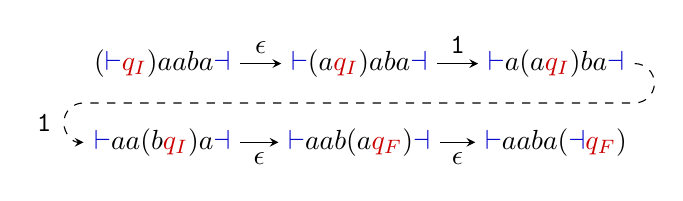
\begin{tikzpicture}[scale=1]
\node (1) at (0,0) {{$({\color{blue!80!black} \vdash}{\color{red!80!black}q_I})  aaba {\color{blue!80!black} \dashv}$}};

\node (2) at (2.5,0) {{$ {\color{blue!80!black} \vdash}  (a{\color{red!80!black}q_I})aba {\color{blue!80!black} \dashv}$}};

\node (3) at (5,0) {{$ {\color{blue!80!black} \vdash}  a(a{\color{red!80!black}q_I})ba {\color{blue!80!black} \dashv}$}};

\node (4) at (0,-1) {{$ {\color{blue!80!black} \vdash}  aa(b{\color{red!80!black}q_I})a {\color{blue!80!black} \dashv}$}};

\node (5) at (2.5,-1) {{${\color{blue!80!black} \vdash}  aab(a{\color{red!80!black}q_F}) {\color{blue!80!black} \dashv}$}};

\node (6) at (5,-1) {{${\color{blue!80!black} \vdash}  aaba ({\color{blue!80!black} \dashv}{\color{red!80!black}q_F})$}};


\draw[->,>=stealth] (1) edge[] node[above] {$\epsilon$} (2) ;
\draw[->,>=stealth] (2) edge[] node[above] {$\mathtt{1}$} (3) ;
\draw[->,>=stealth,dashed] (6,0) arc(90:-90:.25)   -- (-1,-.5) arc(90:270:.25)  ;
\node at (-1.5,-.75) {$\mathtt{1}$};
\draw[->,>=stealth] (4) edge[] node[below] {$\epsilon$} (5) ;
\draw[->,>=stealth] (5) edge[] node[below] {$\epsilon$} (6) ;
\end{tikzpicture}
\end{comment}

\begin{center}

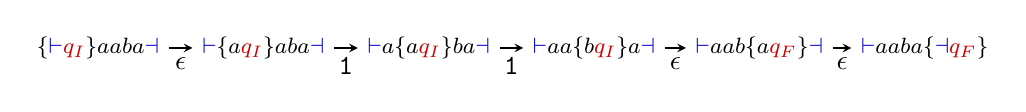
\begin{tikzpicture}[scale=1.05]
\node (1) at (0,0) {\footnotesize{$\{{\color{blue!80!black} \vdash}{\color{red!80!black}q_I}\}  aaba {\color{blue!80!black} \dashv}$}};


\node (2) at (2,0) {\footnotesize{$ {\color{blue!80!black} \vdash}  \{a{\color{red!80!black}q_I}\}aba {\color{blue!80!black} \dashv}$}};

\node (3) at (4,0) {\footnotesize{$ {\color{blue!80!black} \vdash}  a\{a{\color{red!80!black}q_I}\}ba {\color{blue!80!black} \dashv}$}};

\node (4) at (6,0) {\footnotesize{$ {\color{blue!80!black} \vdash}  aa\{b{\color{red!80!black}q_I}\}a {\color{blue!80!black} \dashv}$}};

\node (5) at (8,0) {\footnotesize{${\color{blue!80!black} \vdash}  aab\{a{\color{red!80!black}q_F}\} {\color{blue!80!black} \dashv}$}};

\node (6) at (10,0) {\footnotesize{${\color{blue!80!black} \vdash}  aaba \{{\color{blue!80!black} \dashv}{\color{red!80!black}q_F}\}$}};


\draw[->,>=stealth] (1) edge[] node[below] {$\epsilon$} (2) ;
\draw[->,>=stealth] (2) edge[] node[below] {$\mathtt{1}$} (3) ;
\draw[->,>=stealth] (3) edge[] node[below] {$\mathtt{1}$} (4) ;
\draw[->,>=stealth] (4) edge[] node[below] {$\epsilon$} (5) ;
\draw[->,>=stealth] (5) edge[] node[below] {$\epsilon$} (6) ;
\end{tikzpicture}

\end{center}

\end{example}


\paragraph{Pebble transducers}

In the litterature (see \textit{e.g.}~\cite{Bojanczyk18}), a $k$-pebble transducer is a transducer with $k$ reading heads. The movement of these heads is subject to a stack discipline: only the pebble on top of the stack can move.
In this paper, we will work with a different yet equivalent definition of $k$-pebble transducers. Here a $k$-pebble transducer is a collection of $k$ distinct $1$-pebble transducers. The idea is that the transducer number $k$ can, along its run, call transducer $k-1$ to run over \emph{its} current configuration. Then transducer $k-1$ can itself call transducer $k-2$ to run over its current configuration, and so on. This is analogous of program composition: when a program $A$ calls a program $B$ as a subroutine, first program $B$ is executed on the current state of program $A$, then program $A$ resumes its computation.



\begin{definition}
  A $k$-pebble transducer of input alphabet $\Sigma$ and output alphabet $\Gamma$ is a tuple $\Tt=\atuple{T_1,\dots,T_{k}}$ such that for every $i\in\set{1,\ldots,n}$:
  \begin{itemize}
  \item  $T_i$ is a 1-pebble transducer, whose set of states is denoted $Q_i$;
  \item  The input alphabet of $T_i$ is $\Sigma$ plus predicates in $Q_{>i}\quad$ ($Q_{>i}=\bigcup_{j>i}Q_j$);
  \item  The output alphabet of $T_i$ is $\Gamma \cup \set{\call_1,\ldots,\call_{i-1}}$.
  \end{itemize} 
  In particular, the input alphabet of $T_k$ is $\Sigma$ and the output alphabet of $T_1$ is $\Gamma$.
\end{definition}
The output letter $\call_j$ is to be interpreted as the transducer calling $T_j$ to run over its current configuration.
For every $i\in\set{1,\ldots, k}$,  the sequence $\atuple{T_1,\ldots,T_i}$ can be seen as an $i$-pebble transducer, of input alphabet $\Sigma_i=\Sigma\times \mathbf 2 ^{Q_{>i}}$ and output alphabet $\Gamma$. We denote this transducer by $\Tt_i$.

 \begin{definition}
We define, by induction on $k$, the function realized by a $k$-pebble transducer. The case $k=1$ has been treated in Definition~\ref{def:1pebble}. 

Consider a $k+1$ pebble transducer $\Tt=\atuple{T_1,\ldots,T_{k+1}}$, and let $Q_i$ be the set of states of $T_i$, for $i\leq k$.
By induction let $f_i:\Sigma_i^*\to \Gamma^*$ denote the transduction realized by $\Tt_i$, for $i\in \set{1,\ldots,k}$.
Let us define the image of a word $w$ of $\Sigma^*$ by the transduction realized by $\Tt$:
\begin{itemize}
  \item Let $r=c_1,\ldots,c_{n+1}$ be the accepting run of $T_{k+1}$ over $w$ and $\gamma_1,\ldots,\gamma_n$ be the outputs of the corresponding configurations.
  
  \item  For every $j\in\set{1,\ldots,n}$, let $u_j$ be the word obtained from $\gamma_j$ by replacing each occurrence of a letter $\call_i\in \set{\call_1,\ldots,\call_k}$ by $f_i(c_j')$ (where $c_j'$ is $c_j$ without endmarkers).
  
  \end{itemize}
  The image of $w$ by $\Tt$ is the word $u_1\cdots u_n$.
\end{definition}

\begin{example}
Let us consider the $2$-pebble transducer $\Tt=\tuple{T_1,T_2}$, where $T_2$ realizes a function $f_{\mathrm{pref}}$ similar to the one defined in Example~\ref{ex:prefix}: it makes a number of calls to $T_1$ corresponding the length of the $a$ prefix of the input (separated by $\sharp$ symbols). $T_1$ realizes the transduction $f_{1}:(\set{a,b}\times \mathbf 2 ^{\set{q_I,q_F}})^*\mright \set{a,b}^*$ that copies a word, but erases the state predicates.
Then the transduction realized by $\Tt$ is the function $f:w\mapsto w^{|f_{\mathrm{pref}}(w)|}$.
The function $f$ copies an input word as many times as the length of the prefix of the word with only $a$'s.

The picture below illustrates the behavior of $\Tt$: first $T_2$ runs over the input word, and each time $T_2$ produces a $\call_1$, this is interpreted as a call to $T_1$ to run over the current configuration. 

\begin{center}

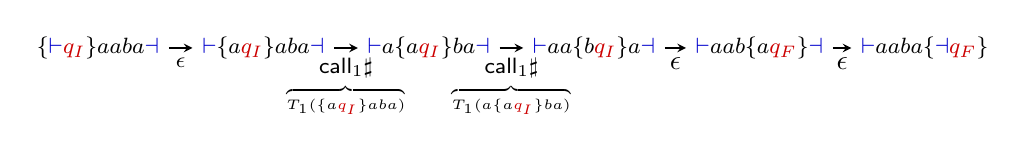
\begin{tikzpicture}[scale=1.05]
\node (1) at (0,0) {\footnotesize{$\{{\color{blue!80!black} \vdash}{\color{red!80!black}q_I}\}  aaba {\color{blue!80!black} \dashv}$}};


\node (2) at (2,0) {\footnotesize{$ {\color{blue!80!black} \vdash}  \{a{\color{red!80!black}q_I}\}aba {\color{blue!80!black} \dashv}$}};

\node (3) at (4,0) {\footnotesize{$ {\color{blue!80!black} \vdash}  a\{a{\color{red!80!black}q_I}\}ba {\color{blue!80!black} \dashv}$}};

\node (4) at (6,0) {\footnotesize{$ {\color{blue!80!black} \vdash}  aa\{b{\color{red!80!black}q_I}\}a {\color{blue!80!black} \dashv}$}};

\node (5) at (8,0) {\footnotesize{${\color{blue!80!black} \vdash}  aab\{a{\color{red!80!black}q_F}\} {\color{blue!80!black} \dashv}$}};

\node (6) at (10,0) {\footnotesize{${\color{blue!80!black} \vdash}  aaba \{{\color{blue!80!black} \dashv}{\color{red!80!black}q_F}\}$}};

\draw[->,>=stealth] (1) edge[] node[below] {\footnotesize{$\epsilon$}} (2) ;
\draw[->,>=stealth] (2) edge[] node[below] {\footnotesize{$\call_1 \sharp$}} (3) ;
\draw[->,>=stealth] (3) edge[] node[below] {\footnotesize{$\call_1 \sharp$}} (4) ;
\draw[->,>=stealth] (4) edge[] node[below] {$\epsilon$} (5) ;
\draw[->,>=stealth] (5) edge[] node[below] {$\epsilon$} (6) ;


\node (2) at (3,-.6) {\tiny{$\overbrace{T_1(  \{a{\color{red!80!black}q_I}\}aba)}$}};

\node (2) at (5,-.6) {\tiny{$\overbrace{T_1( a\{a{\color{red!80!black}q_I}\}ba)}$}};


\end{tikzpicture}

\end{center}
By definition $f_1(  \{a{\color{red!80!black}q_I}\}aba)=f_1(  a\{a{\color{red!80!black}q_I}\}ba)=aaba$, hence we obtain $f(aaba)= aaba\sharp aaba\sharp$.
\end{example}
  

\begin{definition}
  Let $f:\Sigma^*\to \Gamma^*$ be a word to word function.
  We say that $f$ has \emph{degree $k$ growth} (or, abusing notations, that it is \emph{in $\Oo(n^k)$}) if the size of the image of a word of size $n$ is in $\Oo(n^k)$.
  For degrees $0$, $1$ we shall use respectively the terms \emph{bounded} and \emph{linear growth}.
  %Moreover $f$ is \emph{strictly linear} if it is linear and not bounded.
  
\end{definition}


The number of pebbles bounds in an obvious way the degree of a polyregular function:
\begin{proposition}
  \label{prop:degree}
The function realized by a transducer with $k$ pebbles is in $\Oo(n^k)$.
\end{proposition}

\begin{comment}
\begin{proof}
The proof is done by induction on $k$. A $1$-pebble transducer is linear. Let us assume that $k$-pebble transducers are of growth degree $k$. Let  $\Tt=\atuple{T_1,\ldots,T_{k+1}}$ be a $k+1$-pebble transducer. Then $T_{k+1}$ is linear in the number of calls to $\Tt_k$, which means that $\Tt$ is in $\Oo(n\cdot n^k)=\Oo(n^k)$.
\end{proof}
\end{comment}

\section{Results}
\label{sec:results}
We start by stating our results. First, the growth degree characterizes the number of necessary pebbles:
\begin{restatable}[Characterization]{theorem}{onkthm}
    \label{thm:onk}
    A polyregular function is in $\Oo(n^k)$ if and only if it can be realized by a transducer with $k$ pebbles.
\end{restatable}
Moreover, the characterization above is decidable and one can actually minimize the number of pebbles:
\begin{restatable}[Minimization]{theorem}{minthm}
    \label{thm:min}
    Given a polyregular function $f$ one can compute an equivalent pebble transducer with the minimal number of pebbles. In particular, one can decide if a polyregular function is regular.
\end{restatable}
Finally as a consequence (using the result from \cite[Thm.~7]{BojanczykKL19}) we obtain a correspondence between the dimension of \mso interpretations and the number of pebbles of pebble transductions.
\begin{restatable}[\mso-dimension]{theorem}{msothm}
    \label{thm:mso}
    A word-to-word function can be defined by an \mso interpretation of dimension $k$ if and only if it can be realized by a $k$-pebble transducer.
\end{restatable}
We now spend the rest of the article showing the above results. We start by introducing our main tool, the notion of transition morphism of a $1$-pebble transducer. We first characterize the regular functions, then we tackle the general case of degree $k$ growth in the final section.

We show in Sec.~\ref{sec:reg} how to decide if a regular function is bounded.  In Sec.~\ref{sec:poly} we prove the main lemma of the article, Lem.~\ref{lem:name}, which tells, given a $k$-pebble transducer, if one can construct an equivalent $k-1$-pebble transducer.
But first we need to define the notion of transition monoid of a $1$-pebble transducer.


\section{Deciding if a regular function is bounded}
\label{sec:reg}
We start by showing how to decide if a regular function is bounded or not. This not very deep result will serve as a stepping stone for the main contribution of the article.
To characterize bounded regular function, our main tool will be the usual notion of transition morphism of a 1-pebble transducer.

\begin{comment}
    A regular function has at most linear growth, but its output may be smaller than that. Let us show that there is a dichotomy: either a regular function has linear or bounded output size. This is not very hard to see: intuitively, either there is an input word with a part that can be pumped and which produces something, and then the length of the output is linear in the number of times the loop is pumped; or there is no such part, which means that any pumpable part can be removed without changing the output length, hence the output size is bounded.
    This not very deep result will serve as a stepping stone for the main contribution of the article.
\end{comment}

\subsection{Transition morphism of 1-pebble transducers}
We present here the tool used to summarize the behavior of a $1$-pebble transducer, called its transition monoid (resp. morphism). We map each word $w$ to an element of the monoid which gives the following kind of information \textit{e.g.}: if the automaton enters the word from the left in state $q$, then it exits to the left in state $q'$, \textit{etc}.
Moreover, we will sometimes need to record information about the output produced in such a pass of the transducer; this information can be for instance the whole output (in which case the monoid is infinite) or information of the kind ``a letter $a$ has been produced at least once'' (here we recover finiteness).

  
   
\begin{definition}%[Transition monoid of a 1-pebble transducer]
Let $T$ be a 1-pebble transducer with set of states $Q$. Let $N$ be a monoid, and let $\star$ be its multiplication.

We define the transition monoid $M_N$ of $T$ as follows:
\begin{itemize}
\item its elements are functions of the form $f:Q\times\set{\mright,\mleft}\to Q\times\set{\mright,\mleft}\times N$;
\item the composition $\cdot$ is defined as follows. Let $f, g$ be two elements of $M_N$, $q\in Q$ and $d\in\set{\mright, \mleft}$. We define the \emph{transition sequence} between 
$f$ and $g$ starting from $(q,d)$ and its \emph{output sequence} to be respectively the sequences $(q_i,d_i)_{i\in[0,n]}$ and  $(w_i)_{i\in[1,n]}$ satisfying the following conditions: 
\begin{itemize}
\item $(q_0,d_0)=(q,d)$;
\item $d_{n-1}=d_{n}$ and $d_i\neq d_{i+1}$ for every $i\in[1,n-2]$;
\item if $d_0=\mright$ then for every even $i$, $f(q_i,d_i)=(q_{i+1},d_{i+1}, w_{i+1})$ and for every odd $i$, $g(q_i,d_i)=(q_{i+1},d_{i+1}, w_{i+1})$;
\item if $d_0=\mleft$ then for every even $i$, $g(q_i,d_i)=(q_{i+1},d_{i+1}, w_{i+1})$ and for every odd $i$, $f(q_i,d_i)=(q_{i+1},d_{i+1}, w_{i+1})$. 
\end{itemize}
We set $(f\cdot g) (q,d)$ to be $(q_n, d_n, w_1\star\dots\star w_n)$.
\end{itemize}
We give in the picture below an illustration the transition sequence of $f,g$ starting in $(q,\mright)$.
\begin{center}
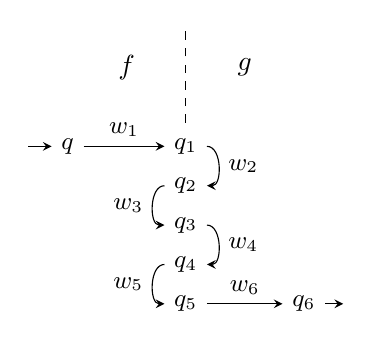
\begin{tikzpicture}
\node[] (0) at (0,0) {\small{$q$}};
\node[] (1) at (1.5,0) {\small{$q_1$}};
\node[] (2) at (1.5,-.5) {\small{$q_2$}};
\node[] (3) at (1.5,-1) {\small{$q_3$}};
\node[] (4) at (1.5,-1.5) {\small{$q_4$}};
\node[] (5) at (1.5,-2) {\small{$q_5$}};
\node[] (6) at (3,-2) {\small{$q_6$}};

\draw[<-,>=stealth] (0) -- node[above] {} (-.5,0);
\draw[->,>=stealth] (0) -- node[above] {\small{$w_1$}} (1);
\draw[->,>=stealth] (1) to[out=0,in=0] node[right] {\small{$w_2$}} (2);
\draw[->,>=stealth] (2) to[out=180,in=180] node[left] {\small{$w_3$}} (3);
\draw[->,>=stealth] (3) to[out=0,in=0] node[right] {\small{$w_4$}} (4);
\draw[->,>=stealth] (4) to[out=180,in=180] node[left] {\small{$w_5$}} (5);
\draw[->,>=stealth] (5) -- node[above] {\small{$w_6$}} (6);
\draw[->,>=stealth] (6) -- node[above] {} (3.5,-2);

\draw[dashed] (1.5,.3) -- (1.5,1.5);
\node[] at (.75,1) {$f$};
\node[] at (2.25,1) {$g$};

\end{tikzpicture}
\end{center}
\end{definition}
We will mainly instantiate $M_N$ in the following three cases: 
\begin{enumerate}
\item $N$ is the monoid $\Gamma^*$ of words over $\Gamma$.
\item $N$ is the two element monoid $\mathbf 2$ with operation $\max$.
\item $N$ is the singleton monoid $\mathbf 1$.
\end{enumerate}
In the last case, the third component of the codomain of the elements of $M_{\mathbf 1}$ is useless, one can be see them as functions of type $Q\times\set{\mright,\mleft}\to Q\times\set{\mright,\mleft}$.


Let us show define the transition morphisms associated with a 1-pebble transducer.
\begin{definition}
Let $T=(\Sigma, \Gamma, Q, q_I, q_F, \delta)$ be a 1-pebble transducer. 
We define the morphism $\mu:(\Sigma_{\vdash\dashv})^*\to M_{\Gamma^*}$ as follows:
$$\text{For every } d\in \set{\mright,\mleft}\qquad\mu(a)(q,d)=\delta(a,q)$$
Let $\Delta\subseteq \Gamma$. We define the morphism $\mu_\Delta:(\Sigma_{\vdash\dashv})^*\to M_{\mathbf 2}$ as follows. Let $\chi_\Delta:\Gamma^*\to \mathbf{2}$ be the morphism defined on letters as follows $\chi_\Delta(\gamma)=1$ if $\gamma\in \Delta$ and $\chi_\Delta(\gamma)=0$ otherwise. We set for every $d\in\set{\mright,\mleft}$: 

$$\text{If } \delta(a,q)=(q',d',w) \text{ then } \mu_\Delta(a)(q,d)=(q',d',1_\Delta(w))$$
We define the morphism $\mu_{\mathbf{1}}:(\Sigma_{\vdash\dashv})^*\to M_{\mathbf 1}$ as follows. For every $d\in\set{\mright,\mleft}$,
$$\text{if } \delta(a,q)=(q',d',w) \text{ then }  \mu(a)(q,d)=(q',d') $$
\end{definition} 

\begin{example}
    Let us consider the transducer given in Ex.~\ref{ex:prefix}.
    Its transition function is:

    $\delta: \begin{array}{crclrcl}
        &(\vdash,q_I) &\mapsto& (q_I,\mright,\epsilon) \\
        &(a,q_I)& \mapsto& (q_I,\mright,\mathtt{1}) & (a,q_F)& \mapsto& (q_F,\mright,\epsilon)\\
        &(b,q_I)& \mapsto& (q_F,\mright,\epsilon) & (b,q_F)& \mapsto & (q_F,\mright,\epsilon)\\
        &(\dashv,q_I)& \mapsto& (q_F,\mright,\epsilon) & (\dashv,q_F)& \mapsto & (q_F,\mright,\epsilon)\\
    \end{array}$

\noindent As an example let us consider $f=\mu_{\set{\mathtt 1}}(ab)=\mu_{\set{\mathtt 1}}(aaababa)$, then $f: (q_I,\mright)$ $\mapsto (q_F,\mright,1)$. This means that the word $ab$ (as well as the word $aaababa$) goes from $q_I$ to $q_F$ from left to right, producing at least on symbol in $\set{\mathtt 1}$.
\end{example}


\subsection{Producing triples and bounded regular functions}
Now that we have defined the transition morphism of a 1-pebble transducer, we can introduce the notion of \emph{producing triple} which characterizes non-boundedness. Intuitively, a producing triple means a loop in the run of the transducer that produces a non-empty output and can thus be pumped to produce arbitrarily large outputs.


\begin{definition}[Producing triple]
Let $T=(\Sigma,\Gamma,Q,q_I,q_F, \delta)$ be a 1-pebble transducer, and let $\Delta\subseteq \Gamma$. Let $(x, e, y)\in \mu_\Delta( { \vdash}\Sigma^*)\times \mu_\Delta( \Sigma^*)\times \mu_\Delta( \Sigma^*{ \dashv})$.

We say that the triple $(x,e,y)$ is \emph{$\Delta$-producing} if the transition sequence of $(xe,ey)$ starting from $(q_0,\mright)$, 
$(q_i,d_i)_{i\in[0,n]}$ satisfies the following conditions:
\begin{itemize}
\item $q_0=q_I$ and $q_n=q_F$;
\item $e$ is idempotent i.e. $e\cdot e=e$;
\item there exists $i\in [1,n-1]$ such that $e(q_i,d_i)$ is of the form $(q,d,1)$.
\end{itemize}
\end{definition}

 \begin{definition}
Let $f:\Sigma^*\to \Gamma^*$ be a function and $\Delta\subseteq\Gamma$. We say that $f$ is bounded (resp. linear, \textit{etc}) in $\Delta$ if $\pi_\Delta\circ f: \Sigma^*\to \Delta^*$ is bounded (resp. linear, \textit{etc}), where $\pi_\Delta:\Gamma^*\to \Delta^*$ is the morphism defined on letters as follows:
\begin{align*}
\pi_\Delta(a)&=a \text{ if }  a\in \Delta \\
&= \epsilon \text{ otherwise.}
\end{align*}
 \end{definition}
The following lemma states that having a producing triple characterizes the functions that are unbounded.
\begin{lemma}\label{thm:linear}
A $1$-pebble transducer is bounded in $\Delta$ if and only if it has no $\Delta$-producing triple.
\end{lemma}
For the proof of the lemma, we will use a notion of factorization in a morphism, which will also be used in Sec.~\ref{sec:poly}.

\begin{definition}
    Let $\mu:\Sigma^*\to M$ be a monoid morphism and let $w$ be in $ \Sigma^*$.
    A $k$-factorization of $w$ in the morphism $\mu$ is given as a tuple of words $(w_0,x_{1},y_1,z_1,w_1,\ldots,x_k,y_k,z_k, w_k)$ verifying:
    \begin{itemize}   
        \item  $w=w_0x_1y_1z_1w_1\cdots x_ky_kz_kw_k$
        \item for all $i\in [1,k]$, $\mu(x_i)=\mu(y_i)=\mu(z_i)=\mu(x_ix_i)$
    \end{itemize}
    We say that such a factorization is \emph{according to} $(m_0,e_1,m_1,\ldots,e_k,m_k)$ if for all $i\in [0,k]$, $\mu(w_i)=m_i$ and for all $i\in [1,k]$, $\mu(x_{i})=e_i$.
\end {definition}

\begin{proof}
    We know that a $1$-pebble transducer realizes a linear function, from Proposition~\ref{prop:degree}.
    Let $T$ be a $1$-pebble transducer realizing a function $f:\Sigma^*\to \Gamma^*$, and let $\Delta\subseteq \Gamma$.

    Let us first assume that there exists a $\Delta$-producing triple $(m_0,e_1,m_1)$, and let $w$ be a word such that ${\vdash} w{\dashv }$ has a $1$-factorization $(w_0,x_1,y_1,z_1,w_1)$ according to this triple.
    Then we show that since $(m_0,e_1,m_1)$ is $\Delta$-producing, $|f(w_0x_1y_1^nz_1w_1)|=\Theta(n)$.
    By definition of $\Delta$-producing triple, the output while reading a $y_1$ factor is non-empty, hence $f$ is strictly linear.

    Let us now assume that there are no $\Delta$-producing triples.
    By a Ramseyan argument, there exists an integer $d$ such that any word of length greater than $d$ has a $1$-factorization.
    Let $w$ be a word with a $1$-factorization $(w_0,x_1,y_1,z_1,w_1)$. Since there are no $\Delta$-producing triple, $(\mu_\Delta(w_0),\mu_\Delta(y_1),\mu_\Delta(w_1))$ is not $\Delta$-producing. This means that the outputs corresponding to the factor $y_1$ in the run over $w$ are all empty, and thus we have $|f(w_0x_1y_1z_1w_1)|=|f(w_0x_1z_1w_1)|$.
    Hence we have $\set{|f(w)|\mid\ w\in \Sigma^*}=\set{|f(w)|\mid\ w\in \Sigma^{\leq d}}$, hence $f$ is bounded.
\end{proof}



\section{Deciding if a polyregular function is in $\Oo(n^k)$}
\label{sec:poly}

Now that we have solved the case of 1-pebble transducers, we move on to general case: deciding if a $k+1$-pebble transduction can be realized by a $k$-pebble transducer. The main idea is, given $\atuple{T_1,\ldots,T_{k+1}}$, to modify $T_{k+1}$ so that it calls $T_k$ only when ``necessary''. Then, if this modified $T_{k+1}$ is bounded in $\set{\call_k}$, it means that the function can actually be realized by a transducer with $k$ pebbles.



\begin{lemma} 
    \label{lem:bounded}
    Let $\atuple{T_1,\ldots,T_{k+1}}$ be a pebble transducer realizing a function $f$, such that $T_{k+1}$ is bounded in $\set{\call_k}$. Then $f$ can be realized by a $k$-pebble transducer.
\end{lemma}     


\begin{lemma}
    \label{lem:precomp}
    Transductions realized by transducers with $k$ pebbles are closed under pre-composition with rational functions.
\end{lemma}


\begin{claim}\label{claim:2idem}
Let $(M,\cdot)$ be a monoid and $\mu:\Sigma^*\to M$ be a morphism. Let $w_1,w_2, w_3\in\Sigma^*$ such that there exits $x,y,z,t,e,f\in M$ satisfying:
\begin{itemize}
\item $\mu(w_1w_2)=x\cdot e$ and $\mu(w_3)=e\cdot y$,
\item $\mu(w_1)=z\cdot f$ and $\mu(w_2w_3)=f\cdot t$,
\item $e$ and $f$ are idempotent.
\end{itemize}
For every $u, v\in\Sigma^*$ such that $\mu(u)=e$ and $\mu(v)=f$ we have that:
\begin{itemize}
\item $\mu(w_1vw_2)=x\cdot e$, 
\item $\mu(w_2uw_3)=f\cdot t$.
\end{itemize}
\end{claim}

\begin{proof}
We have that $\mu(w_1v)=z\cdot f\cdot f=z\cdot f=\mu(w_1)$.
Thus $\mu(w_1vw_2)=\mu(w_1v)\cdot \mu(w_2)=\mu(w_1)\cdot \mu(w_2)=\mu(w_1\cdot w_2) =x\cdot e$.
We proceed in the same way for the other equality.
\end{proof}


\begin{lemma}[Named Lemma]\label{lem:name}
    Let $\Tt=\atuple{T_1,\ldots,T_k}$ be a pebble transducer over input alphabet $\Sigma$ realizing a function $f$.
    There exists a morphism in a finite monoid $\mu:(\Sigma_{\vdash\dashv})^*\to M$ and a set $P\subseteq M^{2k+1}$ such that:
    \begin{itemize}
    \item For any $w\in \Sigma^*$ with a $k$-factorization 
    $(w_0,x_{1},y_1,z_1,w_1,\ldots,x_k,y_k,z_k, w_k)$ according to an element of $P$, $|f(w_1x_1y_{1}^nz_1w_1\cdots x_ky_k^nz_kw_k)|=\Theta(n^k)$.
    \item $f$ restricted to words without $k$-factorization according to any element of $P$ can be realized by a $k{-}1$-pebble transducer.
    \end{itemize}
    
\end{lemma}



\begin{proof}
    This is shown by induction on $k$.
    For $k=1$, it is a consequence of the proof of Lem.~\ref{thm:linear}.

    We assume that the lemma holds for $k$, let us show that it holds for $k+1$.
    Let $\Tt=\atuple{T_1,\ldots,T_k,T_{k+1}}$ be a pebble transducer realizing a function $f:\Sigma^*\to\Gamma^*$, and let $\Tt_k=\atuple{T_1,\ldots,T_k}$. Let $f_k:\Sigma_k^*\to \Gamma^*$ be the function realized by $\Tt_k$.

    Let us apply the induction assumption to $\Tt_k$, and let $\mu:(\Sigma_{k,\vdash\dashv})^*\to M$ and $P$ be given as in the lemma. Let $\Ss$ be a $k{-}1$-pebble transducer realizing the function $f_k$ restricted to words without any $k$-factorization according to elements of $P$, and let $g$ denote the function it realizes.

    The main idea of the proof is to modify the transducer $T_{k+1}$ into a new transducer which only outputs $\call_k$ when it is \emph{absolutely necessary}, \textit{i.e.}~when the word can be factorized in such a way that, by pumping idempotents, one can obtain an output in $\Theta(n^k)$.
    Otherwise, we have according to the lemma that we can outsource the computation to a transducer with only $k-1$ pebbles.

    Let us define a new transducer $R_{k+1}$ which behaves as $T_{k+1}$, except that at each step where it should output the letter $\call_k$, it checks, using some regular look-around if the word has a $k$-factorization according to an element of $P$. If yes then it outputs $k$ normally, calling $\Tt_k$, otherwise it calls $\Ss$ instead.

    The look-around is implemented by a rational function $\ell$ which labels each position by additional information.
    Let $L=Q_{k+1}\to \set{\Ss,\Tt_k}$ be the labelling alphabet, then $\ell:(\Sigma)^*\to (\Sigma\times L)^*$ is defined below:
    Let $w\in (\Sigma)^*$, the word $z=\ell(w)$ has the same size as $w$ and $z[i]=(w[i],h)$ with $h(q)=\Tt_k$ if and only if the word obtained by replacing $w[i]$ with $w[i](q)$ has a $k$-factorization according to an element of $P$.
    Let $\Lambda=\Sigma\times L$ in the following.


    \begin{claim}\label{claim:pump}
        Let $u=\ell(v)$ be in $ \Lambda^*$.
        Let us consider $(w_0,x_1,y_1,z_1,w_1)$ be a $1$-factorization of $v$.
        Let $u_n=\ell(w_0x_1y_1^nz_1w_1)$, then there exists $\alpha,\beta,\gamma\in \Lambda^*$ such that $u_n=\alpha\beta^n\gamma$, for all $n\in \nat$.
    \end{claim}
\begin{proof}[Claim~\ref{claim:pump}]
    Shown using Claim~\ref{claim:2idem}.
\end{proof}
From the above claim, we have that we can pump an idempotent of $M$ without affecting the labelling.
This will not be sufficient however to obtain our final result. We also want to be able to pump an idempotent without changing the \emph{shape} of a run of $R_{k+1}$, that is its transitions without regard to the outputs.
For this we consider the transition morphism $\mu_{\mathbf 1}:(\Sigma_{\vdash,\dashv})^*\rightarrow M_{\mathbf 1}$ of $T_{k+1}$. Indeed, the shape of a run of $R_{k+1}$ over a word $\ell(v)$ is the same as the shape of a run of $T_{k+1}$ over $v$.
Let $\nu=\mu\times \mu_{\mathbf 1}$ denote this product.

Let us consider the $\set{\call_k}$-linear triplets of $R_{k+1}$.
We need to show two things, 1) that the function over words without $\set{\call_k}$-linear triplets can be done by a $k{-}1$-pebble transducer, and 2) that otherwise we can find a $k$-factorization which yields $\Theta(n^k)$ output by pumping idempotents $n$ times.
The first can be obtained from Lemma~\ref{lem:bounded}. The second point is shown using Claim~\ref{claim:pump}.

Finally we show that we can remove the look-ahead, using Lem.~\ref{lem:precomp}, concluding the proof.
\end{proof}

\section{Proofs of the main theorems}

In this section we use the previous lemma to show the results given in Sec.~\ref{sec:results}.
\onkthm*

\begin{proof}
    From Proposition~\ref{prop:degree}, we already have that $k$-pebble transductions are in $\Oo(n^k)$.
    To show the converse we use Lemma~\ref{lem:name}.
    Let $\Tt$ be a $j$-pebble transducer realizing a function $f$ in $\Oo(n^k)$.
    If $j\leq k$ then $f$ can be realized by a $k$-pebble transducer. If $j>k$, then we only need to show that we can obtain a $j-1$-pebble transducer realizing $f$. Using Lemma~\ref{lem:name}, we know there is a morphism $\mu:(\Sigma_{\vdash\dashv})^*\mright M$ and a set $P\subseteq M^{2j+1}$ such that:
    \begin{itemize}
    \item For any $w\in \Sigma^*$ with a $j$-factorization 
    $(w_0,x_{1},y_1,z_1,w_1,\ldots,x_j,y_j,z_j, w_j)$ according to an element of $P$, $|f(w_1x_1y_{1}^nz_1w_1\cdots x_jy_j^nz_jw_j)|=\Theta(n^j)$.
    \item $f$ restricted to words without $j$-factorization according to any element of $P$ can be realized by a $j{-}1$-pebble transducer.
    \end{itemize}
    Since $f$ is in $\Oo(n^k)$, $P$ has to be empty. Thus $f$ restricted to words without $j$-factorization according to any element of $P$ is just $f$. Hence $f$ can be realized by a $j-1$-pebble transducer.

\end{proof}



\minthm*

\begin{proof}
    We only need to show that we can decide if a $k$-pebble transducer realizes a function that can be realized by a transducer with $k-1$ pebbles.

    Let $\Tt=\atuple{T_1,\ldots,T_k}$ be a pebble transducer over input alphabet $\Sigma$ realizing a function $f$.

    Using Lemma~\ref{lem:name}, we know there exists a morphism in a finite monoid $\mu:(\Sigma_{\vdash\dashv})^*\mright M$ and a set $P\subseteq M^{2k+1}$ such that:
    \begin{itemize}
    \item For any $w\in \Sigma^*$ with a $k$-factorization 
    $(w_0,x_{1},y_1,z_1,w_1,\ldots,x_k,y_k,z_k, w_k)$ according to an element of $P$, $|f(w_1x_1y_{1}^nz_1w_1\cdots x_ky_k^nz_kw_k)|=\Theta(n^k)$.
    \item $f$ restricted to words without $k$-factorization according to any element of $P$ can be realized by a $k{-}1$-pebble transducer.
    \end{itemize}
    Here we use the same kind of argument as in the proof of Theorem~\ref{thm:onk}. Either $P$ is non-empty and $f$ is in $\Theta(n^k)$ and thus cannot be realized by a $k{-}1$-pebble transducer, or $P$ is empty and $f$ can be realized by a $k{-}1$-pebble transducer.
\end{proof}


\msothm*

\begin{proof}
\end{proof}



\section*{Conclusion}


\bibliographystyle{alpha}
\bibliography{bib}
\end{document}
